\begin{chapter}{\label{cha:conc}Conclusions and future work}
\section{Conclusions}
In this chapter, we summarise the conclusions of the work presented throughout the thesis, and suggest directions in which the work can be extended in the future. 

In Part I we described the mean-field theory that allows for accurate modelling of a dilute, weakly interacting BEC. We described the GPE, a non-linear Schr\"odinger equation used to model condensates at zero temperature, along with extensions to finite temperature through phenomenological damping and the classical-field method. We also described the theory and practice of various numerical procedures we have used throughout the thesis.

\subsubsection{Classical-like wakes behind elliptical obstacles in Bose-Einstein condensates}
In Chapter \ref{cha:wake} we showed that a 2D or 3D obstacle in the presence of superfluid flow in a Bose-Einstein condensate generates wakes of quantum vortices which resemble those of classical viscous flow past a cylinder or sphere

We demonstrated a key ingredient to produce classical-like wakes: high vortex nucleation rate so that vortices undergo strong interactions with their neighbours rather than being swept away. The role of ellipticity in this chapter was to reduce the critical velocity for vortex nucleation and increase vortex nucleation frequency and density, to facilitate strong interaction between vortices.  

The symmetric wakes produced are similar to those observed in classical flow at low $\Rey$. We showed that they are unstable, forming time-dependent asymmetric structures similar to the B\'enard--von K\'arm\'an vortex street of classical fluid dynamics.

We described several effects relevant to the motion of objects such as vibrating wires, grids and forks in superfluid helium, where the obstacle's ellipticity plays a role which is analogous to rough boundaries \cite{blaz08,brad05}, and described qualitative patterns in the density distribution that could be potentially observed in experimental atomic Bose-Einstein condensates, with moving laser-induced potentials.

\subsubsection{Decay of 2D quantum turbulence in a highly oblate Bose-Einstein condensate}
In Chapter \ref{cha:shin} , we numerically modelled the experimental set up of Kwon {\it et al.} in which the creation and decay of vortices within a BEC~\citep{kwon_moon_14} was experimentally observed. We showed that the system is well described by simulations of the 2D GPE with phenomenological dissipation (despite the system's technically 3D nature). We elucidated the system's experimentally unobserved early stages, showing that vortex clusters form behind a laser-induced obstacle. We demonstrated that early time symmetry breaking causes disorganisation of the vortices and that by the time the obstacle is removed, the vortices are well randomised. We confirmed the occasional appearance of crescent-shaped density features, resulting either from the proximity of vortex cores or from a sound pulse which follows a vortex-antivortex reconnection.

We showed that the vortices decay in a manner which is consistent with the two mechanisms proposed by Kwon {\it et al.} (loss of vortices at the condensate edge due to thermal dissipation and vortex-antivortex annihilation events within the condensate) and fitted the rate equations proposed by Kwon {\it et al.} and Cidrim {\it et al.} to the vortex decay we observed. We concluded that Cidrim's equation fits to the data most favourably, while providing physically realistic values for the decay rates.

\subsubsection{Quasi-classical turbulence and the critical velocity in a quenched Bose gas}
In Chapter \ref{cha:nonequib}, we modelled a finite temperature homogeneous Bose gas. We evolved the classical field from highly non-equilibrium initial conditions, through vortex tangle decay, to thermalized equilibrium states with ranging temperatures and condensate fractions.

We characterised the turbulent vortex tangle by finding a kinetic energy spectrum that demonstrates a {\it lack} of quasi-classical turbulence, and through tracking the vortex line-density over time, we instead found a decay characteristic of ultra-quantum turbulence. We confirmed the result by calculating the velocity correlation function and integral scale to be consistent with ultra-quantum turbulence.

With the resulting equilibrium states we inserted a cylindrical obstacle with Gaussian profile, and ramped up a fluid flow, relative to the gas.  We found that above the critical velocity, vortices are nucleated as wiggly vortex lines, vortex rings, or as a vortex tangle. We demonstrated that the critical velocity decreases with increasing temperature (becoming zero at the critical temperature for condensation) and scales with the square root of the condensate fraction.

\subsubsection{Simulating the rough surface of a ``Floppy Wire''}
In Chapter \ref{cha:afm}, we modelled the rough surface of a real ``floppy wire'' used in helium II experiments through a potential term in the zero temperature GPE and by imposing a flow. The surface of the wire was provided via atomic force microscopy. We performed two-dimensional simulations of the surface at various levels of truncation and a various flow speeds to probe the parameter space.

We observed for various truncations of the 2D wire profile, at flow velocities in excess of the critical velocity for vortex nucleation, the formation of a `boundary layer' of quantum vortices. In each case, for a high enough imposed flow velocity the boundary layer effect ceases and quantum vortices instead fill the box.

We performed large scale 3D simulations, showing the boundary layer effect in 3D. We then measured the velocity profile and demonstrated a qualitatively similar boundary layer velocity profile as in a classical viscous fluid.  Our results suggest that in current helium II experiments the walls of channels which confine the flow of superfluid liquid helium and the surfaces of moving objects such as wires, grids, propellers, spheres may be covered by a thin `superfluid boundary layer' consisting of vortex loops and rings. This is a surprising effect, because in fluid dynamics boundary layers usually arise from viscous forces, 
which in superfluid liquid helium near the temperature of
absolute zero are completely absent.  These findings further illustrate the deep analogies between classical and quantum fluids.

\section{Future work} 
\subsubsection{Other quantum analogues of classical-like wakes}
Many studies of classical viscous flow have been performed over the years. Collections such as Van Dyke's {\it Album of Fluid Motion} \cite{nagib} demonstrate the wide range of flows possible with various obstacle shapes and sizes in both 2D and 3D regimes. As an example, the wakes of rectangular (rather than circular) obstacles and recesses are shown in Figure \ref{fig:dyke-imgs}. Chapter \ref{cha:wake} investigated the classical-like wakes in the simplest case of a cylinder in quantum flow. It would be an extremely interesting direction for future work to attempt to experiment with the more complicated examples of classical flow patterns that exist in the literature. The idea that the behaviour of many quantum vortices collectively reproduces classical physics would suggest that perhaps other analogies of classical fluid wakes exist in the quantum fluid realm. 
\begin{figure}
\centering
    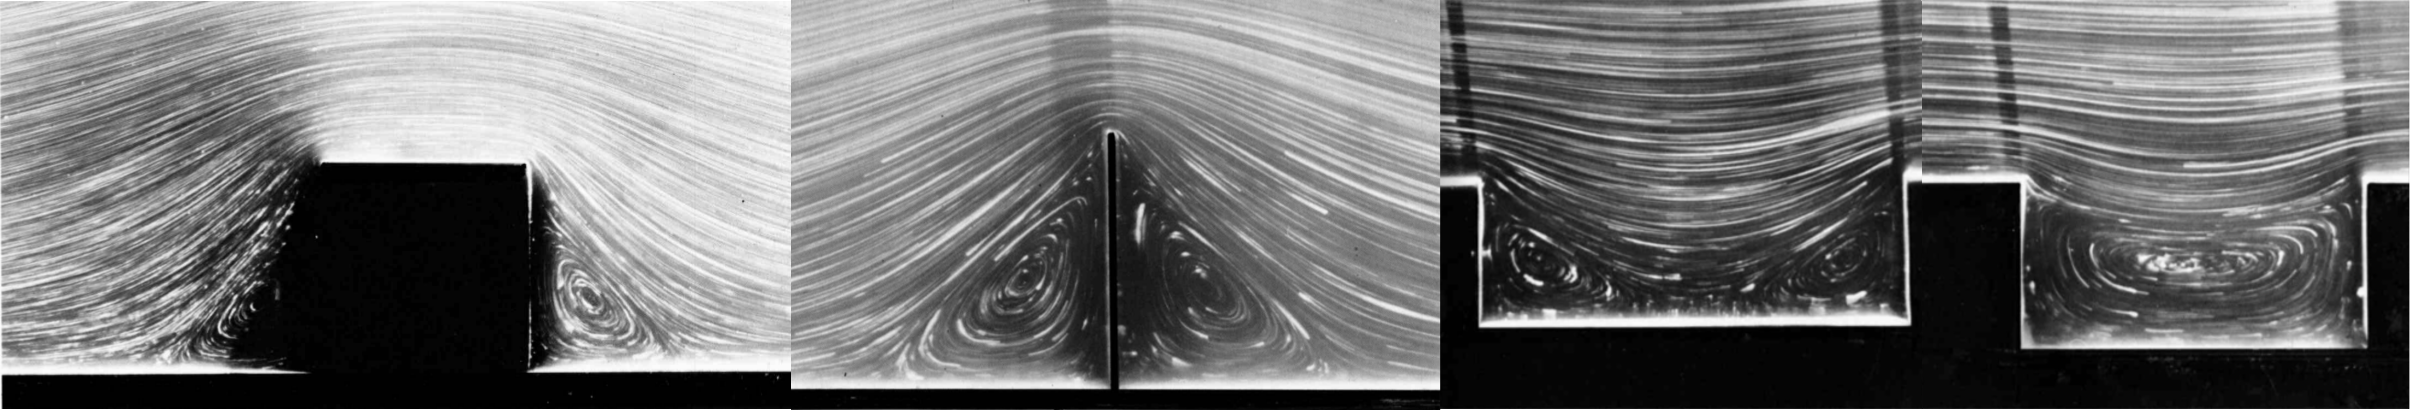
\includegraphics[width=\linewidth]{wake/square.png}
  \caption{Various examples of classical viscous fluid flow around square obstacles and recesses \cite{nagib}.} 
  \label{fig:dyke-imgs}
\end{figure}

\subsubsection{Finite temperature trapped Bose gas}
While the work set our in Chapter \ref{cha:nonequib} is based on a homogeneous system, in reality Bose-Einstein condensates are experimentally confined in traps, rendering the gas inhomogeneous. One can expect significant corrections to the critical velocity due to density gradients, as well as modifications to the vortex nucleation pattern. It would be interesting to see these higher order effects studied in future works, in particular in the common case of a harmonic trapping potential.

On the other hand, recent advances have led to the formation of quasi-homogeneous condensates in box-like traps \cite{gaunt_2013,chomaz_2015}. Here, the higher order corrections associated with trapping inhomogeneity should have minimal effect. An interesting direction for future experimental work would be to compare our experimentally measurable numerical predictions, such as critical velocity or the vortex line-density decay rate, to experimental data incorporating quasi-homogeneous box-like traps.

\subsubsection{Experimentally measuring a superfluid boundary layer}
The experimental implications of possible `superfluid boundary layers`, demonstrated in Chapter \ref{cha:afm}, on macroscopic observables needs to be investigated.  The results we have shown in 2D and 3D should particularly stimulate experiments in $^3$He-B, where, due to relative
large healing length, it is possible to observe vortex core structure and study flows with controlled surface height roughness. 
\end{chapter}